\documentclass[8pt,landscape,a4paper]{scrartcl}

%import
\usepackage[german]{babel}
\usepackage[utf8]{inputenc}
\usepackage{multicol}
\usepackage[landscape]{geometry}
\usepackage{hyperref}
\usepackage{array,multirow,graphicx}
\usepackage{listings}
\usepackage{color}
\usepackage{fancyhdr}
\usepackage{paralist}
\usepackage{tikz}
\usetikzlibrary{decorations.markings}

%define color
\definecolor{sectioncolor}{RGB}{0, 0, 255}
\definecolor{subsectioncolor}{RGB}{0, 100, 255}
\definecolor{subsubsectioncolor}{RGB}{0, 150, 255}
\definecolor{b}{RGB}{0, 120, 255} %Default highlite color
\definecolor{p}{RGB}{0, 43, 54} %Dark page color
\definecolor{t}{RGB}{131, 148, 150} %Dark text color
\definecolor{darkgreen}{RGB}{0,150,0}
\definecolor{dkgreen}{rgb}{0,0.6,0}
\definecolor{gray}{rgb}{0.5,0.5,0.5}
\definecolor{mauve}{rgb}{0.58,0,0.82}

%define code color
\lstset{frame=none,
	language=C,
	aboveskip=0mm,
	belowskip=0mm,
	showstringspaces=false,
	columns=flexible,
	basicstyle={\small\ttfamily},
	numbers=none,
	numberstyle=\tiny\color{gray},
	keywordstyle=\color{blue},
	commentstyle=\color{dkgreen},
	stringstyle=\color{mauve},
	breaklines=true,
	breakatwhitespace=true,
	tabsize=3
}

%define section color and size
\addtokomafont{section}{\color{sectioncolor}\small\rule{5.5cm}{.5pt}\vspace{-2pt}\\}
\addtokomafont{subsection}{\color{subsectioncolor}\small}
\addtokomafont{subsubsection}{\color{subsubsectioncolor}\small}

%define section spacing
\RedeclareSectionCommands[ 
afterindent = false, 
beforeskip = 0pt, 
afterskip = .1pt 
]{section,subsection,subsubsection}

%format
\geometry{top=1.2cm,left=0.4cm,right=0.4cm}

%no section numbers
\setcounter{secnumdepth}{0}

%define header and footer
\pagestyle{fancy}

\fancyhead[RO]{Zindel Marius}
\fancyhead[LO]{CheatSheet Bsys1}
\fancyfoot[RO]{27.01.2020}
\fancyfoot[LO]{Created with \LaTeX}
\renewcommand\headrulewidth{0pt}
\renewcommand\footrulewidth{0pt}
\headsep = -9pt
\footskip = 0pt
\textheight = 563pt

%new commands
\newcommand{\drule}[3][0]{%
	\tikz[baseline]{\path[decoration={markings,
			mark=between positions 0 and 1 step 2*#3
			with {\node[fill, circle, minimum width=#3, inner sep=0pt, anchor=south west] {};}},postaction={decorate}]  (0,#1) -- ++(#2,0);}}

% -----------------------------------------------------------------------




\begin{document}

%------------------Dark Mode----------------	
%\pagecolor{p}
%\color{t}
%------------------Dark Mode----------------


	\begin{multicols*}{5}
		\setlength{\columnseprule}{0.3pt}
		\footnotesize
	\section{Binärdaten I}
	\subsection{Binär / Hex}
		Bit = 1 Gesetztes Bit (set bit) | Bit = 0 Gelöschtes Bit (cleared bit) \\
		\textcolor{b}{LSB} Least Significant Bit, niederwertigstes Bit\\
		\textcolor{b}{MSB} Most Sigificant Bit, höchstwertiges Bit\\
		\textcolor{b}{Nibble} Binärzahl mit 4 Bit\\
		\textcolor{b}{Oktett} Binärzahl mit 8 Bit (\textcolor{b}{== Byte})

	\begin{center}
		\vspace{-8pt}
	\begin{tabular}{|p{0.3cm} p{0.1cm} p{0.3cm} | p{0.2cm} p{0.7cm} p{1.5cm}|}
		\hline
		Binär&Hex&Dez&Pot.& Dez & Dütsch\\
		\hline
		\hline
		0000 & 0 & 0&$2^0$ & = 1 & \\
		0001 & 1 & 1&$2^1$ & = 2 & \\
		0010 & 2 & 2&$2^2$ & = 4 & \\
		0011 & 3 & 3&$2^3$ & = 8 & \\
		0100 & 4 & 4&$2^4$ & = 16 & \\
		0101 & 5 & 5&$2^5$ & = 32 & \\
		0110 & 6 & 6&$2^6$ & = 64 & \\
		0111 & 7 & 7&$2^7$ & = 128 & \\
		1000 & 8 & 8&$2^8$ & = 256 & \\
		1001 & 9 & 9&$2^9$ & = 512 & \\
		1010 & A & 10&$2^{10}$ & = K & $\approx$ 1 Tausend \\
		1011 & B & 11&$2^{20}$ & = M &$\approx$ 1 Million \\
		1100 & C & 12&$2^{30}$ & = G  &$\approx$ 1 Milliarde\\ 
		1101 & D & 13&$2^{40}$ & = T &$\approx$ 1 Billion\\
		1110 & E & 14&$2^{50}$ & = P &$\approx$ 1 Billiarde\\
		1111 & F & 15&&&\\
		\hline
	\end{tabular}
	\end{center}

\section{Prozessor}
Der Prozessor ist mit dem \textcolor{b}{Speicherbus} verbunden und der Speicherbus besteht aus Adressbus, Datenbus und Steuersignale. Der \textcolor{b}{Adressbus} enthält Adresse der Speicherzelle, auf die zugegriffen werden soll. Der \textcolor{b}{Datenbus} enthält Daten, die aus der Speicherzelle gelesen wurde, bzw. geschrieben werden soll. Jeder Prozessor hat eine kleine Menge an Speicher \textcolor{b}{Register}. Mit seinen Bausteinen kann er \textcolor{b}{Operationen} durchführen. \textcolor{b}{Sequenzen} können Hart-codiert im Prozessor oder auf dem Hauptspeicher sein.
\begin{center}
\begin{tabular}{l l l }
	\hline
	Word & 2 Byte & 16 Bit\\
	Doubleword & 4 Byte & 32 Bit\\
	Quadword & 8 Byte & 64 Bit\\
	Double Qword & 16 Byte & 128 Bit \\
	\hline
\end{tabular}	
\end{center}

\section{Hauptspeicher}
\vspace{-6pt}
\begin{multicols}{2}
	Wert an einer Adresse im Hauptspeicher \textcolor{b}{speichern}:
	\begin{compactenum} []
		\item CPU legt Adresse und Wert auf den Speicherbus
		\item Speichercontroller schreibt Wert in Zelle an der Adresse
	\end{compactenum}
	\columnbreak
	Wert von Adresse \textcolor{b}{lesen}:
	\begin{compactenum}[]
		\item CPU legt Adresse auf den Speicherbus
		\item Speichercontroller liest Wert aus und legt sie auf den Speicherbus
		\item CPU liest Wert vom Bus
	\end{compactenum}
\end{multicols}
\vspace{-10pt}
\begin{center}
	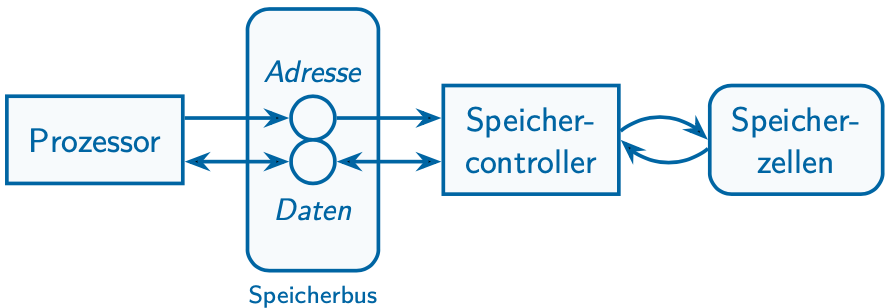
\includegraphics[scale=.3]{Graphic/Speicherbus}
\end{center}
\vspace{-10pt}
\section{Assembler und Linker}
\textcolor{b}{Big-Endian:} \texttt{CAFE$_h$} \textcolor{b}{Little-Endian:} \texttt{FECA$_h$}
\vspace{6pt}
\drule{5.5cm}{1pt}
\begin{center}
	\vspace{-10pt}
	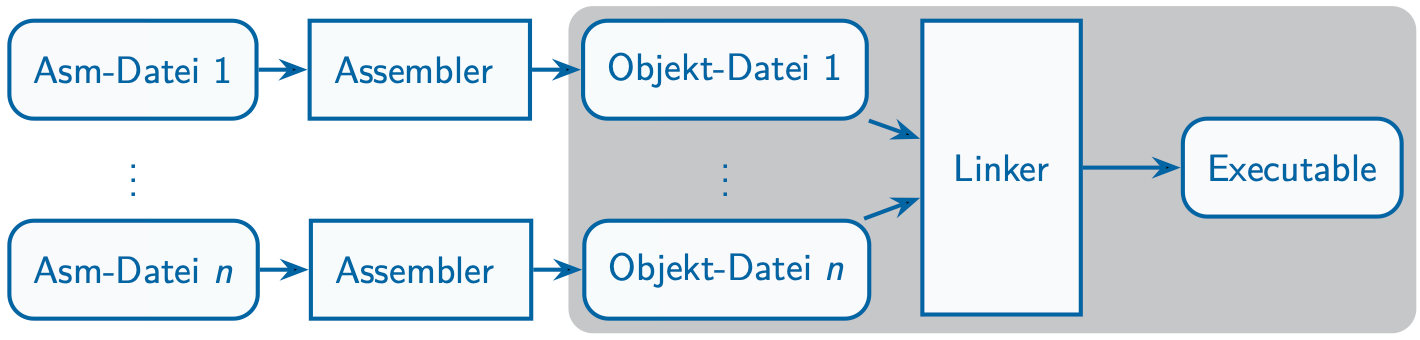
\includegraphics[scale =0.2]{Graphic/Linker}
	\vspace{-4pt}
\end{center}
Programme werden üblicherweise aus mehreren Assemblerdateien generiert.Der Assembler erzeugt aus einer Assemblerdatei eine Objekt-Datei. Der Linker erstellt aus einer oder mehreren Objekt-Dateien ein Executable.
\drule{5.5cm}{1pt}



%\columnbreak



\section{Intel 64 Architektur}
\vspace{-8pt}
\begin{center}
	\begin{tabular}{p{.1cm}|p{.4cm}|p{.4cm}|p{.4cm}|p{.3cm}|p{1.5cm}}
		Nr&64Bit\centering&32Bit&16Bit&8Bit&Beschreibung\\
		\hline
		0&RAX&EAX&AX&AL&Rechenoperat.\\
		\hline
		1&RCX&ECX&CX&CL&Counter für Schleifen\\
		\hline
		2&RDX&EDX&DX&DL&Pointer\\
		\hline
		3&RBX&EBX&BX&BL&Datenpointer\\
		\hline
		4&RSP&ESP&SP&SPL&Stackpointer\\
		\hline
		5&RBP&EBP&BP&BPL&Adresse innerhalb des Stacks\\
		\hline
		6&RSI&ESI&SI&SIL&Zielindizies für Stringoperationen\\
		\hline
		7&RDI&EDI&DI&DIL&Zielindizies für Stringoperationen\\
	\end{tabular}	
\end{center}
\vspace{-8pt}
\textcolor{b}{Datentransfer-Operationen} sind Instruktionen. In ein Register kann man kopieren:
\begin{compactitem} [$\bullet$]
	\item von einem \textcolor{b}{anderen Register}\\
	\texttt{mov rax, rbx}$\rightarrow$Kopiere Inhalt von rax nach rbx
	\item einer \textcolor{b}{Konstante}\\
	\texttt{mov rax, 0x8000}$\rightarrow$Kopiere rax nach $8000_h$
	\item vom \textcolor{b}{Speicher}\\
	\texttt{mov rax, [0x8000]}$\rightarrow$Kopiere Inhalt von rax gleich Inhalt von $8000_h$ ... $8007_h$
\end{compactitem}
\vspace{-4pt}
\drule{5.5cm}{1pt}
Bei \textcolor{b}{Displacement} folgt die Adresse unmittelbar (\texttt{mov rax, [0x800]}).\\
Bei \textcolor{b}{Base} steht die Adresse in einem anderen Register. (mov rax,[rbx])\\
\textcolor{b}{Scaled Index (i * s)}: Index i ist ein Register, Scale s ist eine Konstante (1,2,4 oder 8), die Ausgangsadresse steht in einem Register:\\
$\rightarrow$ \texttt{mov rax, [rcx * 8]}
\vspace{-5pt}
\section{C-Toolchain}
Die \textcolor{b}{Bestandteile} der C-Toolchain sind:\\
C-Präprozessor, C-Compiler, Assembler, Linker\\
Es lassen sich 3 Sprachebenen unterscheiden: 
\begin{compactitem} [$\bullet$]
	\item \textcolor{b}{Präprozessor} definiert Direktiven, die im Programm vor dem eigentlichen
	Übersetzen als Textersetzung durchgeführt werden.
	\item \textcolor{b}{Basiskonstrukte} bestimmen das Grundgerüst eines Programms, z.B. Variablen,
	Schleifen, Verzweigungen.
	\item \textcolor{b}{Standartbibliotheken} stellen Funktionen und Typen bereit, die die Basis-Funktionalität enthalten.
\end{compactitem}
\vspace{-4pt}
\drule{5.5cm}{1pt}
Der \textcolor{b}{Präprozessor} verarbeitet die Datei in mehreren Durchläufen. In jedem Durchlauf wird die ganze Datei bearbeitet.\\
\textcolor{b}{1. Durchlauf:} Entfernt alle Kommentare oder Zeilenumbrüche.\\
\textcolor{b}{2. Durchlauf:} Teilt den gesamten Text in Tokens ein. Es gibt 5 Klassen von Tokens:
\begin{compactenum}
	\item Bezeichner (size\_t)
	\item Präprozessor-Zahlen (0x1234)
	\item String- und Character-Literale (text nach '' oder ')
	\item Operatoren und Satzzeichen (a+++++b $\rightarrow$ a++ ++ +b)
	\item Sonstige
\end{compactenum}
\textcolor{b}{3. Durchlauf:} Durchläuft Token-Liste, führt Präprozessor-Direktiven aus und ersetzt Makros durch Expansion. Ist das erste Token auf einer Zeile \#, wird das nächste Token als Direktive (include, define, if, else, endif) interpretiert.
\drule{5.5cm}{1pt}
Es gibt \textcolor{b}{objektartige} und \textcolor{b}{funktionsartige} Makros. Objektartige Makros haben keine Parameterliste. Der Präprozessor ersetzt im Programm nach der Definition jedes Token, das das dem Makronamen entspricht, durch die Tokenliste.
\textcolor{b}{Tritt} der \textcolor{b}{eigene Makroname in} der \textcolor{b}{Ersetzung} auf, wird er \textcolor{b}{nicht ersetzt}, um infinite Rekursionen zu verhindern.




\columnbreak



\section{Variablen und Zuweisungen}
\textcolor{b}{Deklaration} in C:
\begin{lstlisting}
extern int y; //Es gibt ein int namens y
\end{lstlisting}
\textcolor{b}{Definition} in C;
\begin{lstlisting}
int y = 5; //Reserviert Speicher von int 
//namens y und initialisiert den Wert 5
\end{lstlisting}
Es kann mehrmals Deklariert werden (sofern immmer gleich), jedoch nur einmal definiert!
\drule{5.5cm}{1pt}
\textcolor{b}{Globale Variablen} haben immer einen Typ und Bezeichner. Optional kann jede globale Variabel Initialisiert werden. Sie werden standartmässig exportiert:
\begin{lstlisting}
int c = 5; //in C
global c //in Assembler
c: dd 5 
\end{lstlisting}
Soll eine Globale Variabel aus anderer Objekt-Datei importiert werden:
\begin{lstlisting}
extern int c; //import 
static int c = 5; //wird nicht exportiert!
\end{lstlisting}
\vspace{-8pt}
\begin{center}
	\begin{tabular}{p{1.1cm}p{0.9cm}|p{1cm}p{0.9cm}}
		Bezeichner Obj-Dat. & Deklarat. Assem. & Bezeichner in C & Deklarat. in C\\
		\hline
		lokal & - & global & static\\
		global & global & global & -\\
		- & extern & extern & extern\\
	\end{tabular}
\end{center}
Linker setzt die Dateien auch bei verschiedenen Typen zusammen, da Typen nicht in .o-Dateien gespeichert werden!\\
Lösung: \textcolor{b}{Deklaration} oder \textcolor{b}{Header} erstellen $\rightarrow$ Compiler gibt Fehlermeldung.
\drule{5.5cm}{1pt}
\textcolor{b}{Pointer:} Die Adresse eines Objekts vom Typ T ist vom Typ T*\\
Der \textcolor{b}{Referenzoperator:} \& erzeugt die Adresse eines Ausdrucks.
Der \textcolor{b}{Dereferenzator:} * dereferenziert eine Adresse.
\vspace{-4pt}
\section{Arithmetische und Logische Operationen}
\subsection{logische Operatoren:}
\textcolor{b}{AND ($\wedge$):} Konjunktion\\
\textcolor{b}{OR ($\vee$):} Disjunktion\\
\textcolor{b}{NOT:} Gegenteil\\
\textcolor{b}{XOR ($\bigoplus$):} ==1, wenn a oder b ==1\\
\textcolor{b}{NAND($|$):}==0, wenn a und b ==1\\
\subsection{Zweierkomplement:}
Binärzahl b + N(b) = 0!\\
Vorgehen: b invertieren und + 1 Bit\\
Spezialfall: (0) = 0 und \\
N($2^{n-1}$)= $2^{n-1}$ (für $2^{n-1}$ $<0$)

\subsection{Operationen in C vs. Assembler}
\begin{center}
	\begin{tabular}{p{1cm} | p{1.2cm} | p{2.2cm}}
		Assembler&C&Kommentar\\
		\hline
		add z, q&z = z + q&Addition\\
		sub z, q&z = z - q&Subration\\
		adc z, q&&z=z+q+c(CarryFlag)\\
		sbb z, q&&z=z-q-c\\
		neg z&z=-z&0-z\\
		inc z&z = $++$ z&z+1\\
		dec z&z = $--$ z&z$-$1\\
	\end{tabular}
\end{center}
\subsection{Shiften}
\textcolor{b}{Linksshift} (um 3 Stellen): \\
$101_b * 2^3 = 10'1000_b$ (5$\rightarrow$40)\\
\textcolor{b}{Rechtsshift} (um 3 Stellen):\\
$10'1011_b / 2^3 = 101_b$ (43$\rightarrow$5)\\

\subsection{Multiplikation/Division}
Es dürfen nur signed * signed und unsigned * unsigned gerechnet werden!
\vspace{-4pt}
\begin{center}
	\begin{tabular}{p{1cm} | p{1.2cm} | p{2.2cm}}
		Assembler&C&Kommentar\\
		\hline
		imul z, q&z = z * q&signed Multipl.\\
		mul z, q&z = z * q&unsigned Multipl.\\
		idiv z, q&z = z / q&signed Division\\
		div z, q&z = z / q&unsigned Division\\
	\end{tabular}
\end{center}



%\columnbreak



\section{Kontrollfluss}
\textcolor{b}{Signd} Zahlen $\rightarrow$ Hälfte pos. und neg. Zahlen\\
\textcolor{b}{Unsignt} Zahlen sind nur positiv.\\
Folgende Operationen sind bei beiden gleich:
\begin{compactitem}
	\item Bitoperationen (and, or, xor, not)
	\item Aufgrund des Zweierkomplements (add, adc, sub, sbb, inc, etc.)
\end{compactitem}
Folgende Operationen sind unterschiedlich:
\begin{compactitem}
	\item Multiplikationen (mul (u) / imul (s))
	\item Division (div (u) / idiv (s))
	\item Rechtsschift (shr (u) / sar (s))
\end{compactitem}
\subsection{Division durch Zweierpotenzen C $\rightarrow$ Assembler}
\begin{multicols}{2}
	\begin{lstlisting}
	unsigned ux;
	ux = ux / 8;
	// wird zu:
	mov eax, [ux]
	shr eax, 3
	mov [ux], eax
	\end{lstlisting}
	\begin{lstlisting}
	int sx;
	sx = sx / 4;
	// wird zu:
	mov eax, [sx]
	sar eax, 2
	mov [sx],eax
	\end{lstlisting}
\end{multicols}
\subsection{Flags}
Liegen im Register \texttt{RFLAGS}, das nicht direkt verwendet werden kann.\\
\textcolor{b}{CF - Carry Flag} wird gesetzt, wenn ein Überlauf bei \underline{unsigned} Arithmetik stattfindet.\\
\textcolor{b}{OF - Overflow Flag} wird gesetzt wenn die \underline{Vorzeichen nicht} mehr stimmen.\\
\textcolor{b}{ZF - Zero Flag} wird gesetzt, wenn das Resultat 0\\
\textcolor{b}{SF - Sign Flag} entspricht dem höchstwertigen Bit des Resultats.\\
\textcolor{b}{PF - Parity Flag} wird immer gesetzt, wenn das niederwertigste Byte des Resultats eine gerade Anzahl an gesetzten Bits enthält.
\subsubsection{Condition Codes}
Einige Zustände von Flags oder deren Kombinationen werden als Condition Codes bezeichnet. 
\begin{center}
	\begin{tabular}{p{.5cm}|p{2.3cm}|p{1.5cm}}
		CC&Flags& Info\\
		\hline
		A&CF = 0 and ZF = 0&unsig.: a$>$b\\
		AE&CF = 0&sign.: a$\geq$b\\
		B&CF = 1& unsig.: a$<$b\\
		BE&CF = 1 oder ZF = 1&sign.: a$\leq$b\\
		E&ZF = 1& a = b\\
		G&ZF = 0 and SF = OF&sign.: a$>$b\\
		GE&SF = OF&a$\geq$b\\
		L&SF $\neq$ OF&sign.: a$<$b\\
		LE&ZF = 1 and SF $\neq$ OF&unsig.: a$\leq$b\\
	\end{tabular}
\end{center}
\subsection{Sprünge auf Assembler-Ebene}
\begin{multicols}{2}
	Der Befehl \texttt{JMP d} setzt RIP = RIP + d \underline{nach dem Befehl.} (d ist eine 8- oder 32-Bit-Zahl, die auf 64-Bit-signed extended wird). Anstatt der Zahl \texttt{d} kann auch ein Label verwendet werden.
	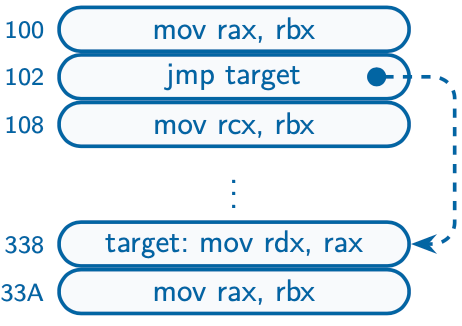
\includegraphics[scale=.34]{Graphic/RelativeSpruenge}
\end{multicols}

\subsection{Iterieren mit Adressen}
In C iteriert man gern direkt mit Adressen. Ein T*-Pointer wird mit ++ um \texttt{sizeof(T)} erhöht. \texttt{int *p = 0x20;} wird nach \texttt{++p} zu \texttt{p == 0x24}
\begin{center}
	
	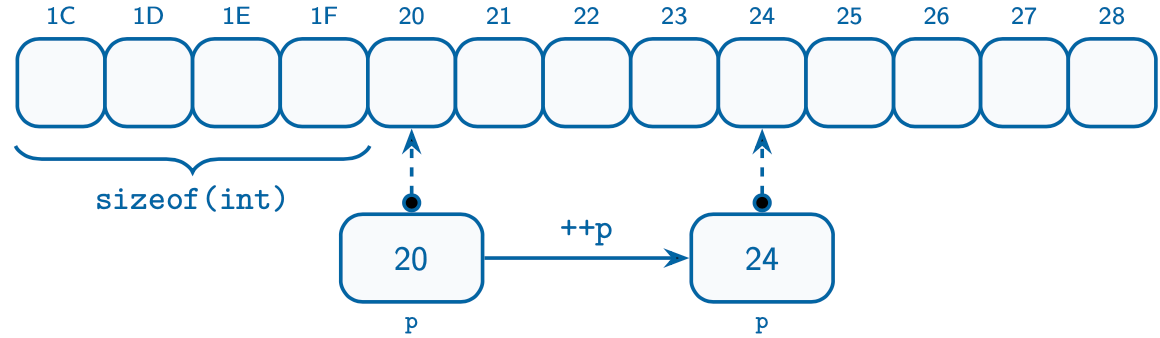
\includegraphics[scale=.27]{Graphic/IterierenAddr}
	
\end{center}



%\columnbreak



\section{Funktionen}
\subsection{Rücksprungmechanismus auf Assembler}
Wird mit \texttt{jmp rsi} umgesetzt. \texttt{rsi} muss jedoch vor dem Springen zum (Label) \texttt{and512} definiert werden.
\subsection{Stackframes und Call-Stack}
Das Konzept «Stack» umfasst einen Stackpointer und Operationen \texttt{push} und \texttt{pop}. \texttt{rsp} zeigt immer auf das zuletzt abgelegte Element.\\
\texttt{push rax} kopiert das Element aus rax auf den Stack und passt den Stackpointer an.
\begin{center}
	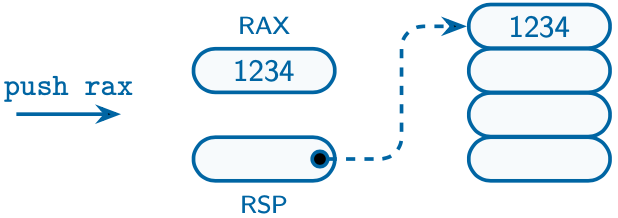
\includegraphics[scale=.35]{Graphic/Push}
\end{center} 
\texttt{pop rax} kopiert das oberste Element vom Stack in rax und passt den Stackpointer an.
\begin{center}
	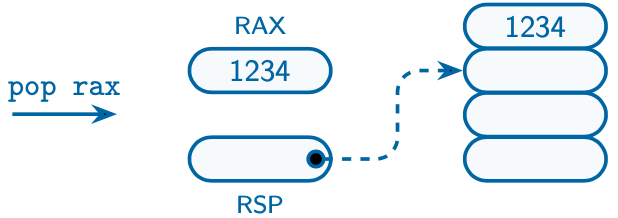
\includegraphics[scale=.35]{Graphic/Pop}
\end{center}

\subsubsection{CALL}
\texttt{call x} legt die Rücksprungadresse auf den Stack und springt dann zu x
\subsubsection{RET}
\texttt{ret} nimmt die Rücksprungadresse vom Stack und springt dahin
\subsubsection{Calling Convention}
Die Calling Convention ist die Vereinbarung zwischen Caller und Callee darüber,
\begin{compactitem} [$\bullet$]
\item wo Argumente / Rückgabewerte übergeben werden: z.B. "Argument 1 liegt in RAX"
\item welche Register die Funktion verändern darf
\item wer den Stackframe für lokale Variablen und Argumente ab- und aufbaut

\end{compactitem}
\subsection{Funktionskonzept in C}
Eine Funktionsdeklaration besteht aus 3 Teilen:
\begin{compactitem} [$\bullet$]
	\item Typ des Rückgabewert (kein Array!)
	\item Bezeichner
	\item Parameterliste in runden Klammern
\end{compactitem}
\subsection{Lokale und Globale Variablen in C}
Jedes Objekt hat in C eine Lebensdauer, während derer Speicherplatz garantiert ist.
\begin{compactitem} [$\bullet$]
	\item \textcolor{b}{Globale Variablen} leben so lange, wie das Programm läuft.
	\item \textcolor{b}{Argumente} leben bis zum Ende der Ausführung der Funktion
	\item \textcolor{b}{Rückgabewert} lebt vom Ende der Funktion bis zur Auswertung des Aufrufers
	\item \textcolor{b}{Variablen} leben vom Zeitpunkt der Definition bis zum Ende des Blocks (\underline{\{\}}), in dem sie definiert wurde.
\end{compactitem}
\subsubsection{Lokale Variabeln}
Variabeln, die innerhalb einer Funktion definiert werden heissen lokal. Sie werden bei jedem Aufruf auf dem Stack oder Register neu angelegt. Werden sie nicht definiert, so ist ihr Wert (im gegensatz zu globalen Variablen) nicht definiert. Adressen lokaler Variablen liegen immer auf dem Stack. Sie können wie jede andere Adresse der Rückgabewert einer Funktion sein, Sie können auch in einen Pointer geschrieben werden.
\subsubsection{Global vs. Lokale Variablen}
\begin{compactitem} [$\bullet$]
	\item Globale Variabeln haben eine fixe Adresse im Speicher
	\item Lokale Variablen werden auf dem Stack angelegt, die Adresse ist nicht fix
	\item Globale Variablen verhindern rekursive Funktionen.
	\item Grundsätzlich können globale sowie lokale Variablen für Zwischenergebnisse verwendet werden
\end{compactitem}



%\columnbreak



\section{Datentypen}
In \textcolor{b}{Assembler} existieren keine Datentypen.\\
In \textcolor{b}{C} gibt es folgende:
\begin{compactitem} [$\bullet$]
	\item \textcolor{b}{\texttt{char}}: Maschinen-Byte
	\item \textcolor{b}{\texttt{int}}: ''natürliche'' Menge an Bits, als signed
	\item \textcolor{b}{\texttt{void *}}: Maschinen-Wort, interpretiert als Addr
	\item \textcolor{b}{\texttt{int *}} Maschinen-Wort, interpretiert als Adresse eines \texttt{int}
\end{compactitem}

Kann nur von gleichen Typen gebildet werden
\begin{lstlisting}
int32_t *y = 100; int 32_t *x = 100;
ptrdiff_t z = x - y; // z ==5
\end{lstlisting}
\subsection{Array}
Die Definition eines Arrays T a[n]; reserviert Speicher für n Elemente vom Typ T und assoziiert das Label a mit der Adresse des ersten Bytes.\\
Arrays werden über eine Liste von Werten in geschweiften Klammern initialisiert.
\begin{lstlisting}
int a[4] = {0x30, 0x10}; //b[2] & b[3] initialized to 0
\end{lstlisting}
Wird nichts in die eckigen Klammern geschrieben, schaut das Array selber, wie gross es sein soll.
\subsection{sizeof(T)}
sizeof a bezeichnet die Anzahl Maschinenbytes des Objekts a. sizeof (T) das gleiche für einen Typ T.
\subsection{Null-terminierte Strings}
Char-Array, deren letztes Element '$\backslash$0' ist.
\subsection{String-Literale}
String Literale stehen zwischen '''', entsprechen einer Sequenz von \texttt{char} und enden mit einer impliziten '$\backslash$0'
\begin{lstlisting}
char * s = "Hai" // gleich wie:
char c[] ={'H','a','i','\0'};char * s =c;
\end{lstlisting}
\subsubsection{\texttt{const}}
\texttt{const} bedeutet, dass der Wert nicht geändert werden darf. Der Wert kann sich aber durch äussere Einflüsse ändern. Am besten von rechts nach links lesen!
\begin{lstlisting}
char const * c; // Pointer to const char
char * const d; // const Pointer to char

++c; 				//OK: c is pointer
++d; 				//ERROR: d is const pointer
*c = 'a';		//ERROR: *c is const char
*d = 'a';		//OK: *d is char
\end{lstlisting}
\subsection{String-Funktionen}
Strings werden in den meisten Fällen als char const * übergeben.
\subsubsection{Strukturierte Variablen}
Globale Variablen können strukturiert werden:
\begin{lstlisting}
stuct{ int x; int y;} t;
\end{lstlisting}
t ist eine strukturierte globale Variable mit den beiden Membern x und y, jeweils vom Typ t. Der Zugriff erfolgt über die Variable t.
\begin{lstlisting}
t.x =5;
\end{lstlisting}
Das erste Member eines Structs hat immer die Adresse wie der Struct selbst. Member müssen nicht dicht liegen, der Compiler darf Padding (Abstände) einfügen.
\subsubsection{Null-Pointer}
Der Int-Wert 0 wird in Verwendung mit Pointer als NullPointer interpretiert.
\begin{lstlisting}
if (px == 0) ... //testet ob Null-Pointer
\end{lstlisting}
\subsubsection{Typ-Casting}
\begin{lstlisting}
int *p = (int *)3; //OK: int 3 cast into pointer
\end{lstlisting}



\columnbreak



\section{Cache}
	\textcolor{b}{Lokalitätsprinzip:} werden bestimmte Daten in kleinen Abständen häufig verwendet, zahlt es sich aus, diese Daten schnell zugreifen zu können. Er funktioniert aber autonom und kann nicht vom Programmierer angesteuert werden. In realen Programmen ist W (t , $\Delta$t ) auch für grössere $\Delta$t konstant.
	 
\subsection{Adressen und Daten im Hauptspeicher}
Hauptspeicher enthält die Adresse \underline{implizit} als Ort der Speicherzelle.
\subsection{Adressen und Daten im Cache}	
Cache muss die (Hauptspeicher-) Adresse \underline{explizit} mit den Daten speichern\\
\drule{5.5cm}{1pt}
\begin{compactitem} [$\bullet$]
	\item \textcolor{b}{Cache-Grösse} Anzahl Nutz-Bytes (ohne Addr.)
	\item \textcolor{b}{Cache-Hit} Gesuchte Adresse ist im Cache
	\item \textcolor{b}{Cache-Miss} Gesuchte Adresse nicht im Cache
	\item \textcolor{b}{$T_c$} Zugriffszeit auf Cache
	\item \textcolor{b}{$T_M$} Zugriffszeit auf Hauptspeicher
	\item \textcolor{b}{$p_c$} Wahrscheinlichkeit eines Hit (oft$>$0.9)
\end{compactitem}
\drule{5.5cm}{1pt}
\subsection{Fully-Associative Cache (FAC)}
Der M-Byte grosse Cache wird in M Einträge aufgeteilt. Eintrag i besteht aus der Adresse $a-i$ und Datenbyte $d_i$
Im Lookup soll überprüft werde, ob der Cache die Adresse a* enthält. Dies wird mit dem Hardwarebaustein c überprüft.
\begin{center}
	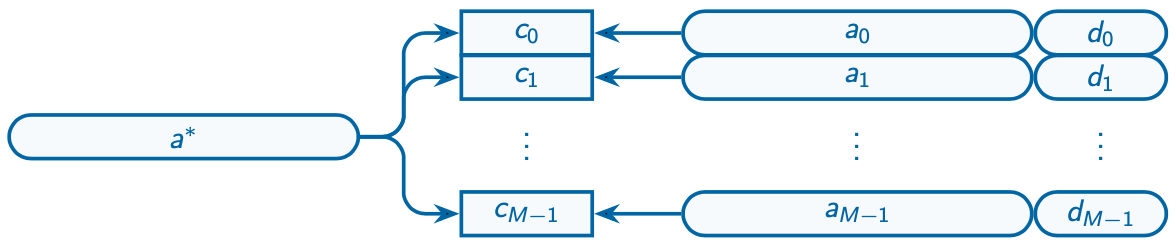
\includegraphics[scale=.25]{Graphic/FAC}
\end{center}
\subsection{FAC mit 64-Byte-Cachezeilen}
Der Cache lädt die Cachezeilen immer als Ganzes. Jeder Cacheeintrag enthält einen \textcolor{b}{Tag $t_k$} und \textcolor{b}{Datenbytes $d_{k,0}...d_{k,63}$}. Die unteren 6 Bits der Adressen in k sind die Zahlen von 0 bis 63. Die oberen n - 6 Bits($\leftarrow$ Tag) sind gleich (Adressen sind n Bit gross).
\begin{center}
	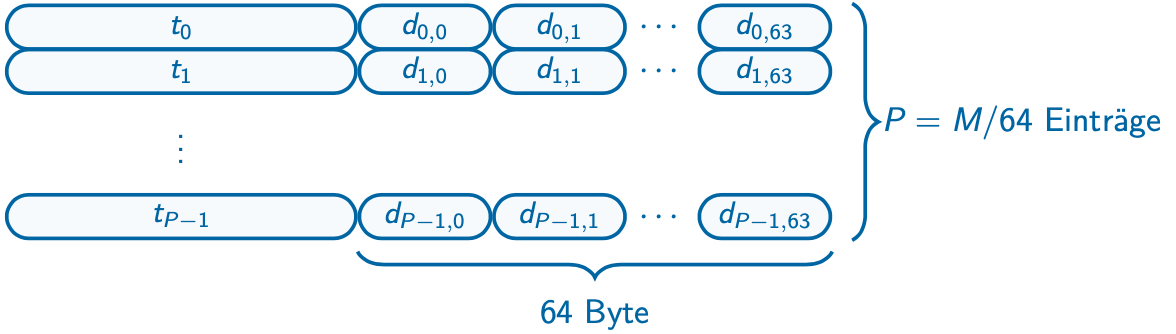
\includegraphics[scale=.25]{Graphic/FAC64}
\end{center}
\subsection{Direct-Mapped Cache (DMC)}
$2^p$ Einträge, die mit p Bits durchnummeriert werden. Eine Cachezeile mit Tag t kann nur einen einzigen Eintrag speichern. Der Teil von t ohne e heisst reduziertes Tag t' = t/$2^p$
\begin{center}
	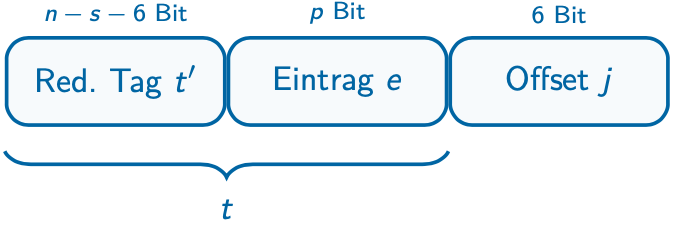
\includegraphics[scale=.36]{Graphic/DMC}
\end{center}
\subsection{k-Way Set-Associative Cache (SAC)}
Ein SAC ist die parallele verwendung von DMCs mit jeweiligen P/k vielen Einträgen. 
\begin{center}
	\vspace{-7pt}
	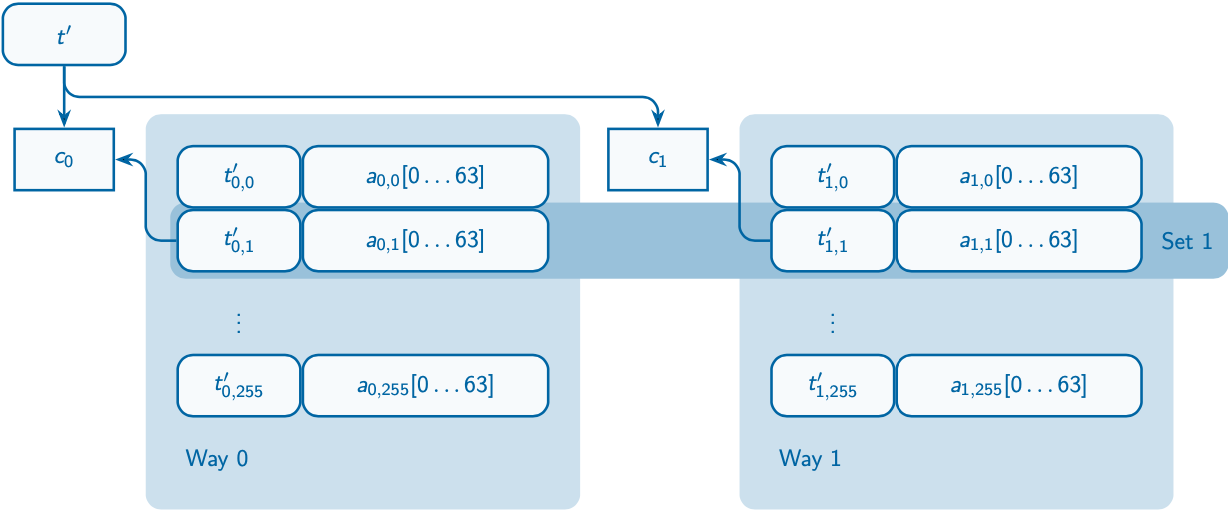
\includegraphics[scale=.2]{Graphic/SAC}
\end{center}	



\columnbreak



\section{Dynamischer Speicher}
Der \textcolor{b}{Heap}:
\begin{compactitem} [$\bullet$]
	\item ist ein Speicherbereich für vollständig dynamischen Speicher
	\item wird vom OS verwaltet
	\item beliebter Zeitpunkt für Reservation / Freigabe
\end{compactitem}
\textcolor{b}{Explizite Speicherfreigabe:} Programmierer definiert, wann Speicher freigegeben wird
\textcolor{b}{Implizite Speicherfreigabe:} Speicher wird automatisch freigegeben, wenn nicht mehr benötigt\vspace{-4pt}\\
\drule{5.5cm}{1pt}
\begin{lstlisting}
void * malloc (size_t s) in <stdlib.h>
\end{lstlisting}
alloziert ein Speicherblock der Grösse s, gibt kleinste verwendbare Adresse zurück und size\textunderscore t ist ein Unsigned-integer für Speichergrösse
\begin{lstlisting}
void free (void *p)
\end{lstlisting}
gibt den Speicherblock frei, der an der Adresse p beginnt.\vspace{-4pt}\\
\drule{5.5cm}{1pt}
\textcolor{b}{Interne Fragmentierung:} Heap-Implementierung reserviert grösseren Speicherblock als benötigt. Zusätzliches Speicherbereich wird vom reservierenden Programm nicht verwendet, kann aber auch für kein anderes Programm verwendet werden. 
\textcolor{b}{Externe Fragmentierung:} Programm reserviert immer wieder Speicher und gibt ihn unregelmässig wieder frei $\rightarrow$ Über längere Zeit entsteht ein Speicherbild, in dem es nur noch kleine Löcher gibt.\vspace{-4pt}\\
\drule{5.5cm}{1pt}
\textcolor{b}{Varianten von Heap-Implementierungen:}
\vspace{-12pt}
\begin{center}
	\begin{tabular}{p{.1mm}|p{4.8cm}}
		\parbox[t]{1mm}{\multirow{24}{*}{\rotatebox[origin=c]{90}{Mehrfache fester Blockgrösse}}} & Implementierung definiert \textcolor{b}{grundlegende Blockgrösse}. Blöcke liegen im Speicher dicht, \textcolor{b}{ohne Zwischenräume}. Grösse des Blocks bestimmt massgeblich die Performance Kleinere Blöcke: mehr Metadaten, langsamer Grössere Blöcke: höhere interne Fragmentierung \\
		&In \textcolor{b}{Bitliste} ein Bit pro Speicherblock: 0$\rightarrow$ Block frei / 1 $\rightarrow$ Block verwendet\\
		&Oder in \textcolor{b}{verketteter Liste} auch möglich:\\
		& \vspace{-13pt}\begin{center}
			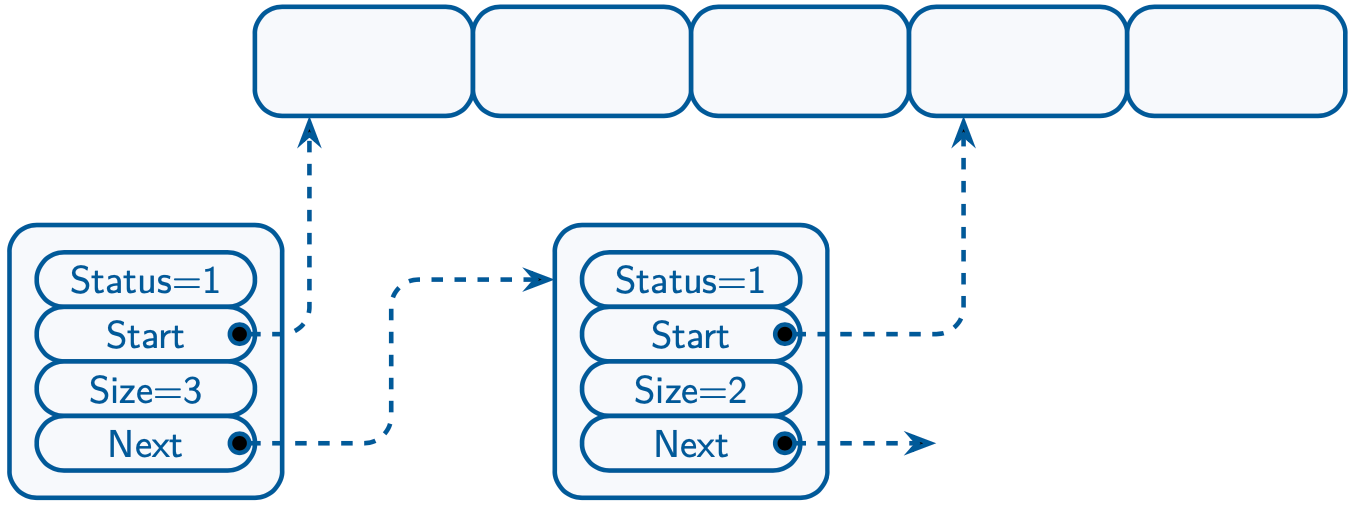
\includegraphics[scale=.2]{Graphic/verketteten_Listen}
			\vspace{-15pt}
		\end{center}\\
		&\textcolor{b}{First Fit:} Wählt erste passende Lücke am Anfang\\
		&\textcolor{b}{Next Fit:} Wählt erste passende Lücke nach zuletzt reserviertem Bereich\\
		&\textcolor{b}{Best Fit:} Durchsucht alle Lücken und wählt die kleinste passende aus\\
		&\textcolor{b}{Worst Fit:} Durchsucht alle Lücken und wählt die grösste aus\\
		\hline
		\parbox[t]{1mm}{\multirow{9}{*}{\rotatebox[origin=c]{90}{Grössenklassen}}} & Bereiche werden nur in \textcolor{b}{bestimmten Grössen} zur Verfügung gestellt, z.B.: Alle Zahlen von 1 bis m. Alle freien Bereiche jeweils einer Grössenklasse werden in jeweils einer Liste vorgehalten.\\
		&\textcolor{darkgreen}{Schnelle Reservation}: Erstes Element aus der Liste der kleinsten passenden Grösse\\
		&\textcolor{red}{Nachteil}: Nachbarn sind nicht leicht zu finden\\
		\hline
		\parbox[t]{1mm}{\multirow{15}{*}{\rotatebox[origin=c]{90}{Buddy-System}}} & Variante des \textcolor{b}{Verfahrens Grössenklassen} mit Zweierpotenzen von $2^m $bis $2^n$. $2^m$ ist die kleinste Speicherbereichsgrösse. $2^n$ ist der gesamte Speicher.\\
		& \vspace{-13pt}\begin{center}
			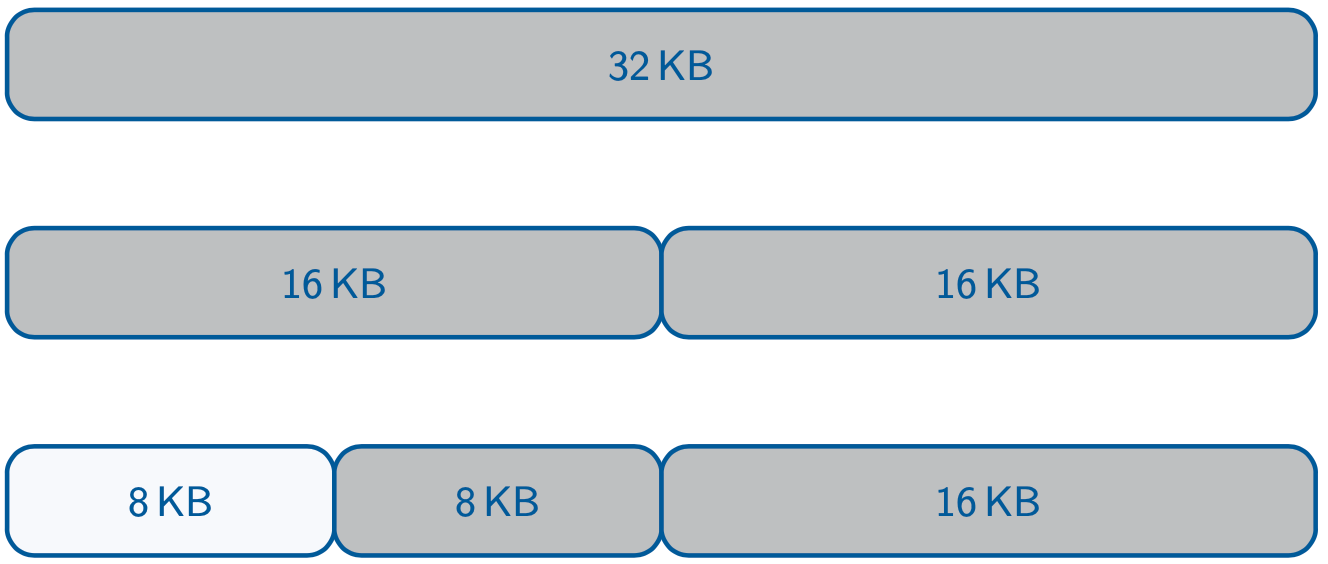
\includegraphics[scale=.15]{Graphic/Buddy}
			\vspace{-8pt}
		\end{center}\\
		&Wird ein $2^k$-\textcolor{b}{Bereich frei}, wird \textcolor{b}{überprüft}, ob sein \textcolor{b}{Buddy in der Freiliste} ist.\\
		&Falls Nein: Bereich in Freiliste einfügen.\\
		&Falls Ja: Entferne Buddy aus Freiliste und Bereich Freigeben.\\
	\end{tabular}
\end{center}



%\columnbreak



\section{Virtueller Speicher}
V-Adresse wird aufgeteilt: PageNr. + Offset\\
FrameNr. + Offset = Reale Adresse\\
Hauptspeicher besteht aus Frames (4KB)\\
V-Adressraum besteht aus Pages (4KB)\vspace{-4pt}
\begin{center}
	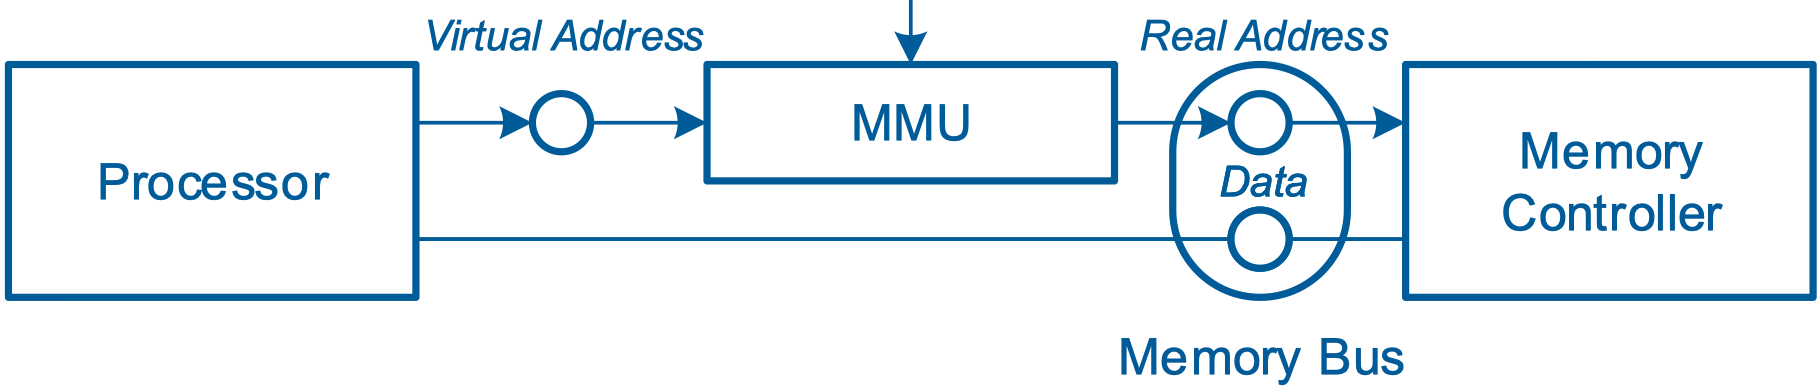
\includegraphics[scale=.17]{Graphic/VAddr}\vspace{-4pt}
\end{center}
Bei ungültiger Adresse $\rightarrow$ MMU stellt fehlendes Mapping fest $\rightarrow$ Fault-Interrupt $\rightarrow$ OS-Interrupt-Handler $\rightarrow$ OS kopiert Pages in RAM und aktualisiert MMU. 
\subsection{Singel Level Page}
\begin{center}
	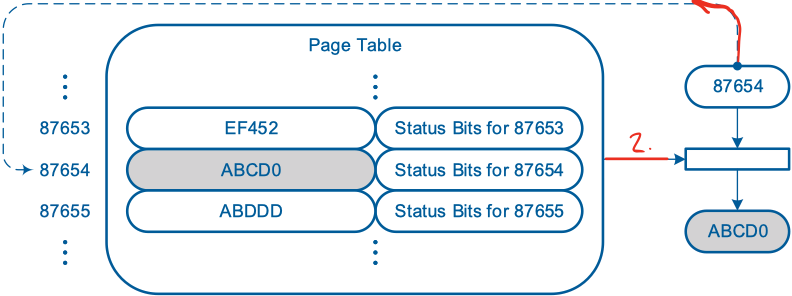
\includegraphics[scale=.25]{Graphic/SingleLevelPage}
\end{center}\vspace{-10pt}
\subsection{Two Level Page}
\begin{center}
	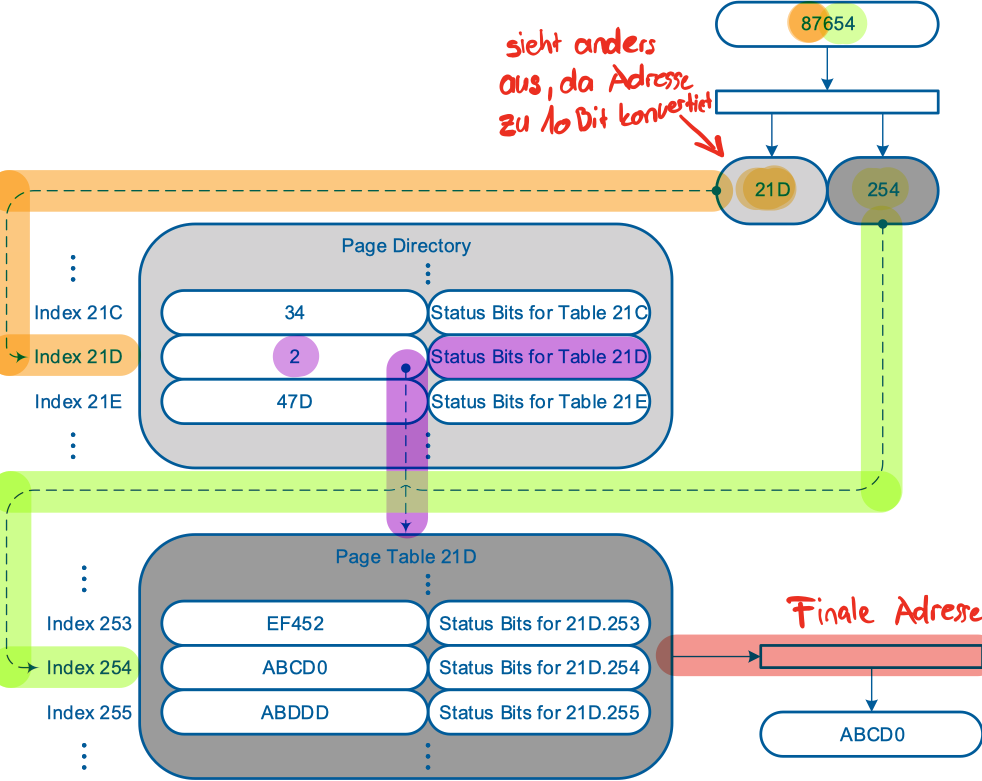
\includegraphics[scale=.22]{Graphic/TwoLevelPage}
\end{center}\vspace{-10pt}
\subsection{Multi Level Page}
Gleich wie Two, nur mit mehreren Hierarchischen Tables (Pointer auf Directory)\\
In einem Page Eintrag gibt es ein \textcolor{b}{Dirty}-Bit,\\
\textcolor{b}{Access}-Bit und \textcolor{b}{P}-Bit (ob im RAM oder nicht)\\
\vspace{-15pt}
\begin{center}
	\begin{tabular}{p{.1mm}|p{4.8cm}}
		\parbox[t]{1mm}{\multirow{9}{*}{\rotatebox[origin=c]{90}{Ladestrategien}}} 
		&\textcolor{b}{Demand Paging} (Laden auf Anfrage)
		\textcolor{darkgreen}{Minimaler Aufwand} / \textcolor{red}{lange Wartezeiten}\\
		
		&\textcolor{b}{Prepaging} (versucht frühzeitig zu laden)
		\textcolor{red}{In Praxis kaum anzutreffen}\\
	
		&\textcolor{b}{Demand Paging mit Prepaging} (Wie D-Paging $+$ benachbarte Page mitladen $\rightarrow$ nach Lokalitätsprinzip) \textcolor{darkgreen}{Weniger Page-Faults / Blocktransfer} / \textcolor{red}{nicht benötigte Pages  werden mitgeladen}\\
		\hline
		
		\parbox[t]{1mm}{\multirow{10}{*}{\rotatebox[origin=c]{90}{Entladestrategien}}}
		&\vspace{-3pt}			
		\textcolor{b}{Demand Cleaning} Entladen auf Anfrage
		\textcolor{darkgreen}{nur geschrieben, wenn nötig} / \textcolor{red}{Erhöhte Wartezeit}\\
		
		&\textcolor{b}{Precleaning} Vorausschauend Schreiben
		\textcolor{darkgreen}{Reduzierte Wartezeit} / \textcolor{red}{Mehr Aufwand}\\
		
		&\textcolor{b}{Page Buffering} (Zwei Listen: Page Numbers der unveränderten Pages / veränderten Pages) MMU setzt D-Bit beim schreiben $\rightarrow$ OS verschiebt dann zu veränderten Pages
			$\pm$ wie \textcolor{darkgreen}{Pre}\textcolor{red}{cleaning}\\
		\hline
		
		\parbox[t]{1mm}{\multirow{22}{*}{\rotatebox[origin=c]{90}{Verdrängungsstrategien}}} 
		&\vspace{-3pt}
		\textcolor{b}{FIFO} (Ersetze jeweils älteste Seite)
		\textcolor{red}{Häufig benutze gelöscht/geladen/gelö/..}\\
		
		&\textcolor{b}{Second Chance} (Prüft A-Bit der Ältesten Seite) ==0$\rightarrow$ weg / ==1 $\rightarrow$ OS löscht A-Bit und schreibt an ende der Liste\\
		
		&\textcolor{b}{Clock} (Wie SC, nur Kreis mit Pointer)\\	
		
		&\textcolor{b}{Least Recently Used} (Page wird grösser $\rightarrow$ HW misst Zeit) \textcolor{red}{MMU kann das oft nicht}\\
		
		&\textcolor{b}{mit Interrupt}( OS misst Zeit $\rightarrow$ R-Bit wird gelöscht nach Timer)\\
		
		&\textcolor{b}{Not Frequently Used} (zusätzliche Counter Table) Pro Eintrag ein Counter. Zugriff: Counter$++$/Löschen: Tiefster Counter\\
		
		&\textcolor{b}{NFU mit Aging}
		\vspace{-4pt}
			\begin{center}
				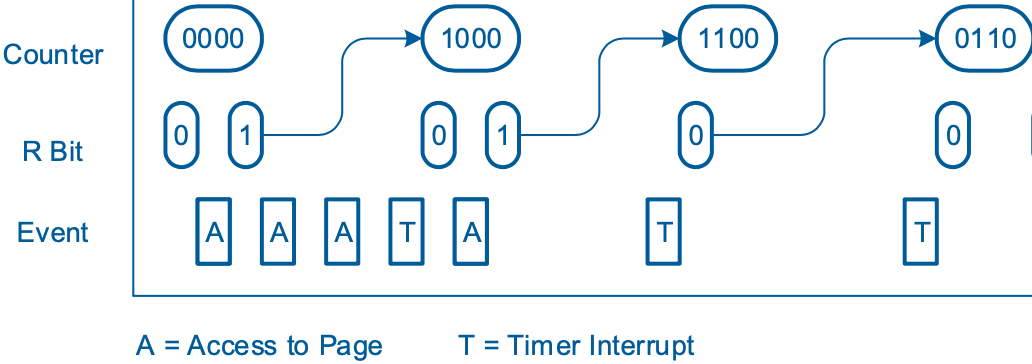
\includegraphics[scale=.24]{Graphic/NFUAging}
			\end{center}\\
	\end{tabular}
\end{center}



%\columnbreak



\section{Ein- und Ausgabe}
Viele Geräte sind Ein- sowie Ausgabegeräte. Deshalb ist die Kommunikation konzeptionell über Register. 
\begin{compactitem}[$\bullet$]
	\item Gerät stellt Register bereit
	\item CPU kann Register lesen oder schreiben
	\item Gerät hat Adress-Pins und Daten-Pins
	\item System hat Adress- und Datenbus
\end{compactitem}
Geräte werden mit einer Schnittstelle verbunden, da direktes verdrahten mit der CPU zu aufwändig wäre.\vspace{-7pt}
\begin{center}
	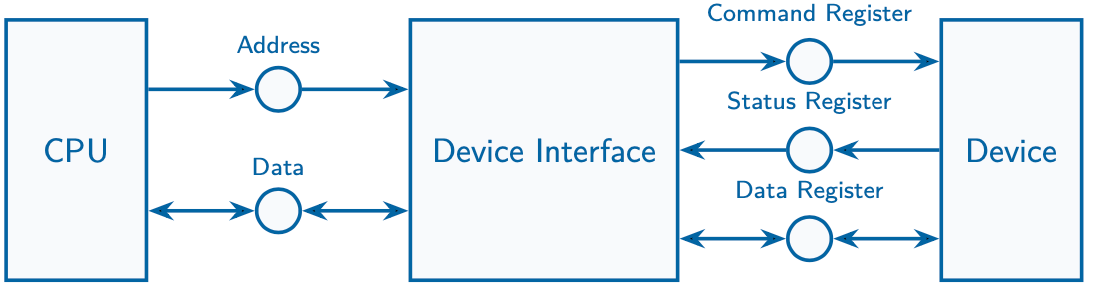
\includegraphics[scale=.25]{Graphic/EinAus}
	\vspace{-10pt}
\end{center}
\textcolor{b}{Memory-mapped I/O}: Jedes Gerät ist am Speicherbus und bekommt einen reservierten Adressbereich. Dieser Bereich kann nicht für Speicher verwendet werden. \textcolor{darkgreen}{CPU} muss \textcolor{darkgreen}{keine Logik} haben / nicht wissen was Geräte sind. \textcolor{red}{Adressraum des Speichers} kann \textcolor{red}{nicht für Speicher verwendet} werden. \\
\textcolor{b}{Port-mapped I/O}:Geräte haben einen separaten Bus und Adressräume. Die CPU hat dann zwei Adressräume und pro Raum eigene Instruktionen. \textcolor{darkgreen}{Speicherverwendung} / \textcolor{red}{Komplexität}\\
\textcolor{b}{Port-mapped I/O via Speicherbus}: Geräte sind am Speicherbus, der aber eine zusätzliche Bitleitung hat. Diese gibt an, ob für Speicher oder I/O. (Etwas von beidem der anderen 2)
\subsection{Kommunikationsmechanismen}
\textcolor{b}{Polling (Programmgesteuert)}: Dies ist ein einfacher Mechanismus: CPU fragt regelmässig das Gerät. Programm pollt Statusregister. Wenn OK $\rightarrow$ Programm kann schreiben/lesen
\textcolor{b}{Polling mit Busy Wait}: Software pollt hintereinander weg. \textcolor{darkgreen}{keine Verzögerung} / \textcolor{red}{legt CPU lahm sehr unprofessionell}\\
\textcolor{b}{Polling ohne Busy Wait}: Software pollt in regelmässigen Abständen gemäss einem vordefiniertem Zeitintervall. \textcolor{darkgreen}{Arbeiten an anderen Aufgaben möglich} / \textcolor{red}{erfordert genaue zeitliche Analyse}\\ 
\textcolor{b}{Interruptgesteuert}: Die Idee ist es, dass das Gerät die Software unterbricht (sendet Interrupt), sobald es bereit ist. Die CPU prüft nach (fast) jeder Instruktion, ob Interrupt Pin gesetzt ist. Falls ja:\\
Unterbricht normale Ausführung $\rightarrow$ Sichert Instructor-Pointer und Kontext (auf dem Stack) $\rightarrow$ holt sich die Nummer n des Interrupts $\rightarrow$ springt zum Interrupt-Handler, der an Index n in der Interrupt Vector Table notiert ist $\rightarrow$ CPU fährt mit der Aufgabe wieder fort.
\textcolor{b}{Direct Memory Access (DMA)}: Die Idee ist es, dass das Gerät direkt auf den Speicher zugreift. Dafür benötigt es zusätzlich einen DMA-Controller. Der Controller steuert den Speicherbus anstelle der CPU. Aus CPU-Sicht ist es nur ein weiteres Gerät.
\begin{center}
	\vspace{-5pt}
	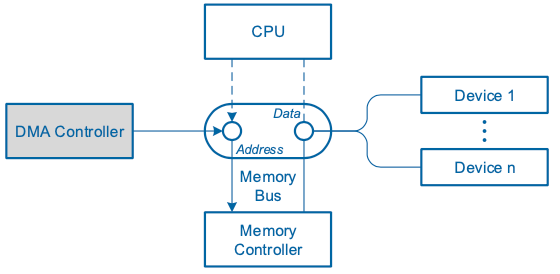
\includegraphics[scale=.5]{Graphic/DMA}
	\vspace{-5pt}
\end{center}

\begin{compactenum} [1.]
	\item CPU programmiert DMA für Transfer: Quelle, Ziel, Menge, Betriebsart
	\item CPU gibt Speicherbus an DMA frei
	\item DMA lässt Gerät direkt in Speicher kopieren
	\item DMA legt Adresse auf Speicherbus
	\item Gerät legt Daten auf Speicherbus
	\item Nach Beendigung setzt DMA Interrupt
\end{compactenum}



	\end{multicols*}
\end{document}}
